%%%%%%%%%%%%%%%%%%%%%%%%%%%%%%%%%%%%%%%%%
% Stylish Article
% LaTeX Template
% Version 2.1 (1/10/15)
%
% This template has been downloaded from:
% http://www.LaTeXTemplates.com
%
% Original author:
% Mathias Legrand (legrand.mathias@gmail.com) 
% With extensive modifications by:
% Vel (vel@latextemplates.com)
%
% License:
% CC BY-NC-SA 3.0 (http://creativecommons.org/licenses/by-nc-sa/3.0/)
%
%%%%%%%%%%%%%%%%%%%%%%%%%%%%%%%%%%%%%%%%%

%----------------------------------------------------------------------------------------
%	PACKAGES AND OTHER DOCUMENT CONFIGURATIONS
%----------------------------------------------------------------------------------------

\documentclass[fleqn,10pt]{SelfArx} % Document font size and equations flushed left

\usepackage[english]{babel} % Specify a different language here - english by default

\usepackage{lipsum} % Required to insert dummy text. To be removed otherwise

\usepackage{enumitem}

%----------------------------------------------------------------------------------------
%	COLUMNS
%----------------------------------------------------------------------------------------

\setlength{\columnsep}{0.55cm} % Distance between the two columns of text
\setlength{\fboxrule}{0.75pt} % Width of the border around the abstract

%----------------------------------------------------------------------------------------
%	COLORS
%----------------------------------------------------------------------------------------

\definecolor{color1}{RGB}{0,0,90} % Color of the article title and sections
\definecolor{color2}{RGB}{0,20,20} % Color of the boxes behind the abstract and headings

%----------------------------------------------------------------------------------------
%	HYPERLINKS
%----------------------------------------------------------------------------------------

\usepackage{hyperref} % Required for hyperlinks
\hypersetup{hidelinks,colorlinks,breaklinks=true,urlcolor=color2,citecolor=color1,linkcolor=color1,bookmarksopen=false,pdftitle={Title},pdfauthor={Author}}

%----------------------------------------------------------------------------------------
%	ARTICLE INFORMATION
%----------------------------------------------------------------------------------------

\JournalInfo{TSBK03 - Teknik för avancerade datorspel\\
             December 15, 2017} % Journal information
\Archive{} % Additional notes (e.g. copyright, DOI, review/research article)

\PaperTitle{Marching cubes sculpt} % Article title

\Authors{
	Adam Söderström\textsuperscript{1}, 
    Oscar Komulainen\textsuperscript{2},
    }

\Keywords{Marching cubes --- WebGL --- Procedurall terrain generation    }
\newcommand{\keywordname}{Keywords} % Defines the keywords heading name



%----------------------------------------------------------------------------------------
%	ABSTRACT
%----------------------------------------------------------------------------------------

\Abstract{
Blyat
		  ~ \\
          \textbf{Source code}: https://github.com/adamsdm/TNM095\vskip -6pt ~ \\ 
          \textbf{Authors}\\
          \textsuperscript{1}\textit{Media Technology Student at Linköping University, adaso578@student.liu.se}\\
          \textsuperscript{2}\textit{Media Technology Student at Linköping University, oscko391@student.liu.se} \\
          \vskip -19pt ~ 
}

%----------------------------------------------------------------------------------------

\begin{document}

\flushbottom % Makes all text pages the same height

\maketitle % Print the title and abstract box

\tableofcontents % Print the contents section

\thispagestyle{empty} % Removes page numbering from the first page

%----------------------------------------------------------------------------------------
%	ARTICLE CONTENTS
%----------------------------------------------------------------------------------------

\section{Introduction} % The \section*{} command stops section numbering

%% \addcontentsline{toc}{section}{Introduction} % Adds this section to the table of contents
\subsection{Machine learning}
The idea that a machine can learn and improve is not a new concept. As early as 1959, S. Arthur wrote: \textit{"Machine learning is a field of computer science that gives computers the ability to learn without being explicitly programmed."} \cite{SamArthur}. However during the time, the computers computational power was very limited, and it would take many years before machine learning would have an actual use and rise in popularity. 
Many of the machine learning techniques require a lot of computational power to deliver a decent result within a reasonable amount of time, and depending on the problem, a lot of training time and training data. With todays modern CPU's this is no longer a problem. The performance can also further be increased by utilizing GPGPU operations, such as CUDA \cite{cuda}, OpenCL \cite{opencl} or compute shaders \cite{computeshader}, the GPU can perform general computation which may drastically outperform the CPU in many cases. 

As late as 2015, Google's DeepMind released their artificial intelligence AlphaGo \cite{alphago} which gave a huge rise in popularity for artificial intelligence. AlphaGo uses a combination of machine learning and tree search techniques to learn how to play the very advanced game Go, and in March 2016, AlphaGo beat the professional Go player Lee Sedol. Later in 2017, DeepMind developed an AI that taught itself how to walk without any knowledge about how humans walk which also gained a lot of attention. \cite{deepmindWalking}

The machine learning technique this paper will discuss is called reinforcement learning. More specifically, the technique Q-learning, and how Q-learning can be used to train an agent to learn how to play the popular game Snake. 

\subsection{Snake}
Snake is a game that was very popular in the early 21st century. It was one of the preinstalled games on the popular phone Nokia 3310. The idea of the game is very simple. The player controls a snake which can move up, down, left or right. Food spawns on the playing field, which if the snake eats, respawns in a different location and the length of the snake grows. The goal of the game is to eat as much food as possible, the player looses if the snake hits itself, or a wall.

%------------------------------------------------
\section{Theory}
Q-learning is a model-free reinforcement learning technique. It is based on the idea to give an agent a reinforcement every time it performs an action. If the agent performs an action that the programmers have specified to be positive, the agent will receive a reward and correspondingly it gets a negative reinforcement when it performs an action that is specified to be negative. 

Q-learning is based on a Q-matrix, where each row corresponds to a state and each column corresponds to an action. The Q-matrix acts as the agents memory of all state and action combinations. States corresponds to the game state. The Q-matrix initial configuration when it starts is either a zero matrix or random values. Anytime the agent takes an action the Q-matrix is updated according to equation \ref{eq:q-learning algo}
\begin{equation}
\label{eq:q-learning algo}
Q(s,a) = (1 - \alpha) \cdot Q(s,a) + \alpha (R(s,a,s') + \gamma maxQ(s',a'))
\end{equation}

Where $s$ is the current state and $a$ is the action. $s'$ corresponds to the next state and $a'$ are the actions possible for the next state. $\alpha$ is the learning rate. If the learning rate is set to zero the Q-matrix will never update and if it is set 1, the agent will maximize the learning rate by only considering the most recent information. $Q$ is the Q-matrix, $s$ is the state and $a$ is the action. $s'$ and $a'$ corresponds to the next state and action. $R$ is the reward matrix which specifies which actions are good/bad in the current state. $\gamma$ is the discount factor, it corresponds to how much the agent will consider the future rewards. \cite{Q-learning-OG} 


%------------------------------------------------
\section{Method} \label{sec:method}

\subsection{Feasability study} \label{subsec:feasabilityStudy}
At the start of the project, the group didn't know what programming language and technique to be used for the AI. Thus, a technical feasibility study was made conducted to find a suitable method for this kind of problem. Previously in the course, a similar AI had been developed to play the game AgarIO using Q-learning \cite{AgarIO}. Since this problem was similar to our, an AI that learns how to play a fairly simple game, the Q-learning method was chosen. Another project in this course used Q-learning to implement an agent for a platform game. This report \cite{platformgame} was also read to gain a better understanding of Q-learning.

The choice of programming language fell on Python, since it provides many AI modules. Two core third party modules that was used in the development of the AI:
\begin{description}
\item[PyGame \cite{pygame}] - PyGame is a third party module  which as the name suggests is a lightweight game engine for python. The base snake game was developed using PyGame.
\item[NumPy \cite{numpy}] - NumPy is a module which allows for creation, manipulation and usage of matrices, and more advanced mathematical structures than the basic operators. It is the most popular module for scientific calculation and utilizes C to achieve much higher performance than vanilla python code. 
\end{description}

\subsection{Implementation}
The first step in the implementation was to create the base Snake game. As mentioned in \ref{subsec:feasabilityStudy}, this was done in PyGame. Since no group member was fluent in Python and PyGame, this took longer than expected. The base game was a very simple grid based 2D-game where the user controls the snake with the arrow keys.

\begin{figure} 
	\centering
		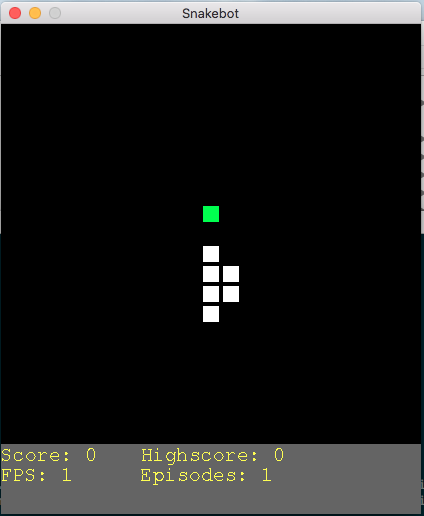
\includegraphics[width=8cm]{basegame.png}
	\caption{The Snake base game implemented in PyGame}
    \label{fig:snakegame}
\end{figure}

As seen in the lower right part of figure \ref{fig:snakegame}, the number of episodes is saved and kept track of. The number of episodes is the number of games that the AI has played. This makes it easier to see how the AI develops as the number of episodes increase.

Once the base snake game was developed, the group was ready to start working on the actual Q-learning. To keep the AI part somewhat independent and more general so that it could be used for similar projects, the AI part was very loosely coupled to the base game. The AI bot is capable of :
\begin{enumerate}[label=\roman*]
  	\item Get observations from the world, determining what state it is in.
	\item Make decisions based on what state the agent is in.
	\item Update the agents memory in order to make better decisions when faced with the same situation.
\end{enumerate}
Every time an action is performed, the Q-matrix is updated.

The learning rate $\alpha$ was initially set to 0.7. This means that initially, actions will have a higher impact on the Q-matrix. This basically means that the AI will learn faster initially. However, after a while once a lot of actions have been performed and reviewed future actions should have a smaller impact. Thus, the learning factor $\alpha$ is decreased over time at a linear rate.

The state is determined from a feature vector which contains the variables blocked left/up/down/right and the direction of the snake. Since these variables can be combined (except for the direction) there are 64 different states. One convenient way to represent a state is by using 8 bits. The first four bits represent blocked up, left right, down. The last 4 bits represent direction of the snake in the same directional pattern. So e.g if the snake is blocked left and right, and it's direction is up, the state could be represented by the bits $01101000$ = 104. I.e the state of the world can be represented by a single integer which was implemented in this implementation. This representation of the states is more maintainable and less computationally heavy than using if-statements to determine the state.

The snake also has a chance to a random action in order to explore more states and get out of loops. This random chance is sometimes called epsilon. It is set to 0.05 at the start and is gradually lowered to 0.01.

%------------------------------------------------

\section{Result} \label{sec:result}

Our result is a bot that learns the environment, but not as much as we expected. It can clearly be seen that the snake learns to avoid running into itself in some simple situations, but it often traps itself by blocking all possible escape routes. It rarely runs into a wall, since this is a simpler problem than running into itself.

The snake is still quite good though, and since it is a machine playing and not a human, it has instant reflexes. It can't however see into the future so a human could still easily outperform the AI. Aswell as mentioned in section \ref{sec:method}, the snake only perceives the world closest to the snake's head, while a human player can see the entire playing field, giving the human an unfair advantage.
%------------------------------------------------

\section{Discussion}
\subsection{Review} \label{subsec:review}
As discussed in section \ref{sec:result}, the snake bot often traps itself i.e. ending up in a situation where there is no escape route. This is probably due to the fact that the bot does not look far ahead on future states. It only looks at the current state and the next state and evaluate what move is the best according to the experience it has gathered during runtime. For example, if the bot has been in a situation where it is running into itself, it must choose to take either a right turn or a left turn in order to survive. Let us say that it chooses a left turn and that it survives in this case, shown in figure \ref{fig:snaketrap1}. The next time the bot is going to run into itself it knows that a left turn was successful the last time and therefore it will choose a left turn again, but in this case it might be in the situation shown in figure \ref{fig:snaketrap2} which means that the left turn results in the snake trapping itself. 

\begin{figure}
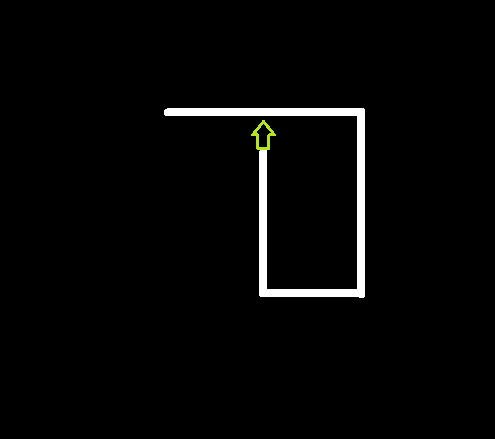
\includegraphics[width=8cm]{SnakeTrap1.png}
\caption{In this case, a left turn will be the correct choice since the snake will not trap itself.}
\label{fig:snaketrap1}
\end{figure}

\begin{figure}
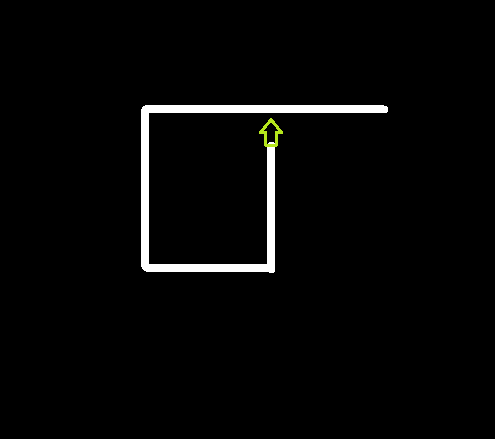
\includegraphics[width=8cm]{SnakeTrap2.png}
\caption{In this case, a left turn will be the wrong choice since the snake will trap itself.}
\label{fig:snaketrap2}
\end{figure}

When researching methods to solve this problem, we found a similar project where the states were represented by a screenshot of the whole playing field which means the snake can see the whole environment. \cite{deep-q-snake} This could possibly solve our problem with the snake trapping itself, but the method would bring some constraints with it. If a state would be represented with a screenshot, the size of the play field would be very limited, since we have to avoid having too large states. For example if the play field is 200x200 pixels large, the Q-matrix matrix would have to include all possible positions and lengths of the snake, as would the reward matrix need to match this Q-matrix. Thus, this solution would not scale very well since the size of the Q-matrix and reward matrix would scale exponentially.

The agent could potentially also be improved by adding more features, e.g. a heuristic which would depend on the path to the food. This could improve the agents behavior in terms of trapping itself.

One of the most difficult tasks in the implementation was what to set the initial reward values and $\alpha$ and $\gamma$. We used a try and error approach to find the optimal starting values for these variables. The values of the reward matrix were also difficult to get right. For example, if the value of running in to a wall was set too low, the agent seemed to take longer to learn to avoid the wall. Likewise if the reward for eating food was set too low the agent would not risk going for the food and instead just avoid death by moving in a a safe circle. If the reward was set too high the agent would put itself in risky situations just to get the food. What was done in this implementation was to set the reward of the food differently depending on what state the snake was in. If the snake was not blocked in any direction the reward for food was set to a higher value. This was done by setting the value for eating food, given the state where the snake was blocked, in the reward matrix.

The group implemented two ways of initializing the Q-matrix, as a zero-matrix and as random values. It was found that setting the Q-matrix to all zeros got a better result in the end, but it was a bit slower to explore the different states in the start. A problem with the random matrix was that it was difficult to tweak the values of the reward matrix to get rid of the randomness at later stages. The Q-matrix initialized as zeros was chosen as the most effective way to initialize the Q-matrix.

\subsection{Q-learning for this kind of problem}
\label{subsec:other techniques}
Although the AI that was developed in this implementation works and learns from it's previous actions as expected, Q-learning might not be the best choice for this kind of problem. Another choice of deep learning technique for this kind of problem could e.g be a CNN (Convolutional Neural Network), which would take a much longer time to train to get a decent result, but could outperform the Q-learning AI developed in this implementation. An implementation of this technique would make an interesting comparison to the Q-learning agent implemented in this project.

Since snake is such a simple game, Q-learning is a bit of an overkill. A technique such as Decision Tree's could be used to outperform the Q-learning AI developed in this implementation.

\subsection{Future work}
\label{subsec:future work}
As discussed in section \ref{sec:result}, the final AI was not able to beat the entire game (i.e fill the entire playing field with the snake, until the snake eats its own tail). This problem is difficult, if not impossible, to solve by simplifying the state as much this implementation did. To develop a AI that would be able to solve the entire game, the state would have to be much more complex. As mentioned in section \ref{subsec:review}, a complete state of all possible world states would have to be saved. This would make the state very large, but this could be solved by limiting the playing field and making it smaller. Another problem, apart from memory, is that the reward matrix would have to be generalized in some way to match the Q-matrix. As of now the reward matrix has been manually initialized with values that represents each state and action pair. The feature vector could also be expanded to create more states and make the agent more aware of its surroundings. Since the number of states grow exponentially with the number of features the problem again becomes that the reward matrix needs to be generalized in order to enable the developers to tweak the reward values. 

%------------------------------------------------

\section{Conclusion}
In order to make the agent better more states would have to be added, either as adding in more features to the feature vector or saving all possible states as screen-shots. The advantage of using a feature vector is that it is a more general approach, and the only way the to save states if the game-world is sufficiently big or even infinite. 

Other machine learning techniques might prove more useful for this specific problem. Especially if  the goal is to make the snake fill the entire grid. 

The values of alpha and gamma as well as the values of the reward matrix could still be tweaked to find optimal values to make the agent perform slightly better. But adding more states is what would have the biggest impact on this implementation.


%----------------------------------------------------------------------------------------
%	REFERENCE LIST
%----------------------------------------------------------------------------------------
\phantomsection
\bibliographystyle{unsrt}
\bibliography{sample}

%----------------------------------------------------------------------------------------

\end{document}